%!TEX root = ../report.tex
\documentclass[report.tex]{subfiles}
\begin{document}
\chapter{Evaluation and Results}

\section{Experiment Description}

We evaluate image matching and clustering performance across two local feature descriptors and two matchers, namely: \textbf{Descriptors} - SIFT and DISK (\(2048\) max keypoints per image), \textbf{Matchers} - FLANN and LightGlue. For the four combinations formed, we aimed to create a single pipeline that extracts features, matches image pairs, clusters images into scenes, and evaluates cluster quality against ground-truth scene labels. We report purity of the clusters formed and its error rate across datasets.

% \section{Implementation Details}
% - Descriptors were capped at \(2048\) keypoints per image for computational reasons.
% -  FLANN: KD-Tree index (\texttt{trees=5}), \texttt{checks=50}, Lowe's ratio test with \(\text{ratio}=0.7\).
% - LightGlue: Default configuration for the selected descriptor supported through LightGlue repository as a sub-module; GPU used when available.
% - 

\section{Clustering and Evaluation}
Image pairs are matched and aggregated into clusters per dataset. Clusters are serialized as JSON with cluster IDs and member image filenames. These cluster files along with ground-truth labels are used for evaluation providing:
\begin{itemize}

    \item Scene-level precision/recall/F1 via greedy scene-to-cluster assignment for each dataset.
    \begin{itemize}
        \item Precision (scene-level): Fraction of images in the chosen cluster that truly belong to the scene.
        \item Recall (scene-level): Fraction of the scene’s images captured by the chosen cluster.
        \item F1 (scene-level): Harmonic mean of precision and recall for the chosen cluster per scene.
    \end{itemize}
       \item  Cluster quality evaluation: 
       \begin{itemize}
           \item Homogeneity: Each cluster contains only members of a single class; [0, 1], 1 = perfectly pure clusters.
           \item Completeness: All members of a class are assigned to the same cluster; [0, 1], 1 = no class is split across clusters.
       \end{itemize}

\end{itemize}


We report the post-clustering evaluation results, outlining each metric, how it was computed, and why it was selected to assess complementary aspects of cluster quality.

\subsection{Per-Dataset Scene Assignment Metrics}
Table \ref{tab:scene-agg-methods} reports precision, recall, and F1 computed by assigning each scene to the cluster that maximizes F1 (ties broken by precision then recall). Table \ref{tab:per-dataset-methods} expands on the  Table \ref{tab:scene-agg-methods} to provide a detailed overview of the metrics over each sub-dataset for all four combinations of the methods.

The results indicate that DISK + LightGlue and SIFT + LightGlue generally perform better than the FLANN-based methods, particularly in terms of recall and F1 scores.

\begin{itemize}
    \item     DISK + LightGlue achieves the highest overall F1 score (0.664) and recall (0.598), as shown in Table \ref{tab:scene-agg-methods}. This suggests it's the most balanced and effective method for capturing all images belonging to a scene while maintaining reasonable precision.
    \item     SIFT + LightGlue is a close second with an F1 score of 0.635 and a high recall of 0.577. This combination is a strong competitor, demonstrating that SIFT, when paired with a robust matcher, can still be very effective.
    \item DISK + FLANN shows the highest precision (0.912) but the lowest recall (0.371). This indicates that while its clusters are very pure (they rarely mix scenes), they are also highly fragmented. This is reflected in the low completeness scores in Table \ref{tab:quality-per-dataset}.
    \item     SIFT + FLANN provides a balanced but lower performance compared to the LightGlue methods, with an F1 score of 0.586. Its recall is significantly lower than the LightGlue-based methods, suggesting it struggles to group all images from a single scene together.
\end{itemize}

\begin{table}
\centering
\begin{tabular}{lrrr}
\toprule
 & Precision & Recall & F1 \\
Method &  &  &  \\
\midrule
SIFT + FLANN & 0.843 & 0.494 & 0.586 \\
SIFT + LightGlue & 0.773 & 0.577 & 0.635 \\
DISK + FLANN & 0.912 & 0.371 & 0.478 \\
DISK + LightGlue & 0.829 & 0.598 & 0.664 \\
\bottomrule
\end{tabular}
\caption{Per-method averages over entire dataset for scene-wise F1/Precision/Recall}
\label{tab:scene-agg-methods}
\end{table}

\begin{table}
\centering
\begin{tabular}{lrrrrrr}
\toprule
 & \multicolumn{3}{r}{SIFT + FLANN} & \multicolumn{3}{r}{SIFT + LightGlue} \\
 & Precision & Recall & F1 & Precision & Recall & F1 \\
Dataset &  &  &  &  &  &  \\
\midrule
ETs & 0.667 & 0.385 & 0.488 & 0.333 & 0.200 & 0.250 \\
amy\_gardens & 1.000 & 0.345 & 0.513 & 1.000 & 0.560 & 0.718 \\
fbk\_vineyard & 0.795 & 0.251 & 0.381 & 1.000 & 0.677 & 0.786 \\
imc2023\_haiper & 0.505 & 0.478 & 0.429 & 0.505 & 0.522 & 0.468 \\
imc2023\_heritage & 0.933 & 0.320 & 0.474 & 0.604 & 0.388 & 0.422 \\
imc2023\_theather\_imc2024\_church & 0.981 & 0.690 & 0.766 & 0.882 & 0.640 & 0.652 \\
imc2024\_dioscuri\_baalshamin & 1.000 & 0.406 & 0.572 & 0.657 & 0.387 & 0.486 \\
imc2024\_lizard\_pond & 0.880 & 0.281 & 0.405 & 0.743 & 0.441 & 0.548 \\
pt\_brandenburg\_british\_buckingham & 0.662 & 0.667 & 0.664 & 1.000 & 1.000 & 1.000 \\
pt\_piazzasanmarco\_grandplace & 1.000 & 0.692 & 0.814 & 1.000 & 0.655 & 0.790 \\
pt\_sacrecoeur\_trevi\_tajmahal & 0.667 & 0.667 & 0.667 & 1.000 & 1.000 & 1.000 \\
pt\_stpeters\_stpauls & 1.000 & 0.770 & 0.851 & 0.495 & 0.500 & 0.498 \\
\bottomrule
\end{tabular}
\vspace{5em}
\begin{tabular}{lrrrrrr}
\toprule
 & \multicolumn{3}{r}{DISK + FLANN} & \multicolumn{3}{r}{DISK + LightGlue} \\
 & Precision & Recall & F1 & Precision & Recall & F1 \\
Dataset &  &  &  &  &  &  \\
\midrule
ETs & 0.667 & 0.352 & 0.460 & 0.619 & 0.385 & 0.473 \\
amy\_gardens & 1.000 & 0.060 & 0.113 & 1.000 & 0.375 & 0.545 \\
fbk\_vineyard & 1.000 & 0.197 & 0.322 & 1.000 & 0.700 & 0.806 \\
imc2023\_haiper & 0.857 & 0.359 & 0.505 & 0.704 & 0.505 & 0.540 \\
imc2023\_heritage & 0.750 & 0.150 & 0.249 & 0.625 & 0.369 & 0.383 \\
imc2023\_theather\_imc2024\_church & 1.000 & 0.293 & 0.451 & 1.000 & 0.700 & 0.786 \\
imc2024\_dioscuri\_baalshamin & 1.000 & 0.232 & 0.370 & 0.660 & 0.408 & 0.497 \\
imc2024\_lizard\_pond & 1.000 & 0.159 & 0.267 & 0.837 & 0.433 & 0.532 \\
pt\_brandenburg\_british\_buckingham & 1.000 & 0.938 & 0.967 & 0.662 & 0.667 & 0.664 \\
pt\_piazzasanmarco\_grandplace & 1.000 & 0.466 & 0.628 & 1.000 & 0.785 & 0.863 \\
pt\_sacrecoeur\_trevi\_tajmahal & 0.667 & 0.667 & 0.667 & 1.000 & 1.000 & 1.000 \\
pt\_stpeters\_stpauls & 1.000 & 0.585 & 0.738 & 1.000 & 1.000 & 1.000 \\
\bottomrule
\end{tabular}
\caption{Per-dataset scene-wise averages for different method}
\label{tab:per-dataset-methods}
\end{table}


\subsection{Scene–Cluster Overlap per Dataset}
These plots visualize how predicted clusters align with ground-truth scenes across datasets and methods. Each point at (cluster ID, scene) represents the number of images shared; marker size encodes overlap (fraction per scene), and color denotes the method (SIFT+FLANN, SIFT+LightGlue, DISK+FLANN, DISK+LightGlue). This highlights scene purity, fragmentation (scenes split across many clusters), and mixing (clusters containing multiple scenes). Better clustering appears as large markers concentrated in one cluster per scene and minimal cross-scene mixing. Some of the plots in Figure \ref{fig:scene-cluster-D} for different datasets are presented below, rest are included in Appendix \ref{appendix:A2}.

\begin{itemize}
    \item  LightGlue-based methods consistently show larger, more concentrated markers , especially in datasets like \texttt{pt\_sacrecoeur\_trevi\_tajmahal} and \texttt{pt\_brandenburg\_british\_buckingham}. This indicates high completeness, where most images from a scene are correctly grouped into a single cluster. For example, in \texttt{pt\_sacrecoeur\_trevi\_tajmahal}, all four methods achieve a perfect V-Measure of 1.000, which is visually represented by the large markers aligned perfectly with a single cluster ID for each scene.
    \item  FLANN-based methods often show a pattern of multiple smaller markers for a single scene across different cluster IDs. For example, in \texttt{imc2023\_haiper} , SIFT + FLANN and DISK + FLANN show fragmentation across multiple clusters for the fountain and chairs scenes. This visually demonstrates the low recall and completeness scores observed in the tables \ref{tab:per-dataset-methods} and \ref{tab:quality-per-dataset}.
    \item The plots also highlight purity vs. fragmentation. DISK + FLANN, with its high precision and homogeneity, forms many pure, small clusters. This is visible in plots like \texttt{imc2023\_theather\_imc2024\_church}, where the DISK + FLANN markers are spread out, indicating many small, distinct clusters.
\end{itemize}

% \begin{figure}
% \centering

% \begin{minipage}{\textwidth}
% \centering
% 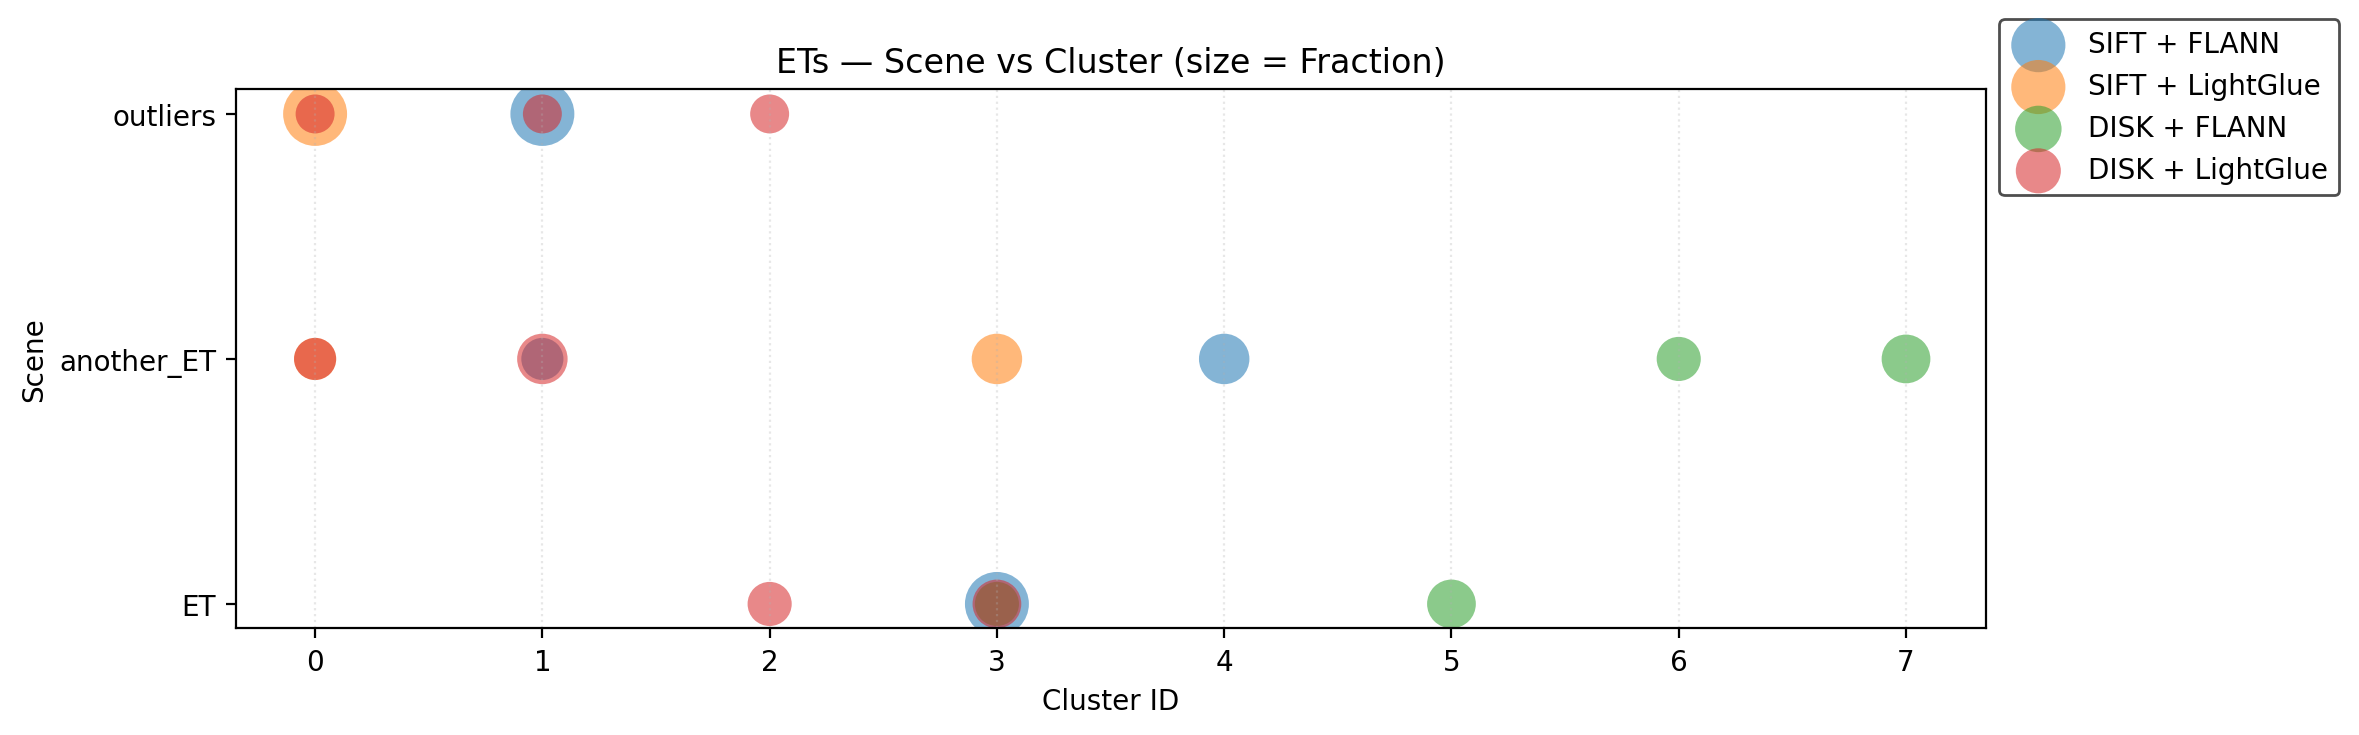
\includegraphics[width=\linewidth]{images/scene_cluster_by_dataset/ETs.png}
% \subcaption{Dataset: ETs}
% \label{fig:scene-cluster-A}
% \end{minipage}
% \begin{minipage}{\textwidth}
% \centering
% 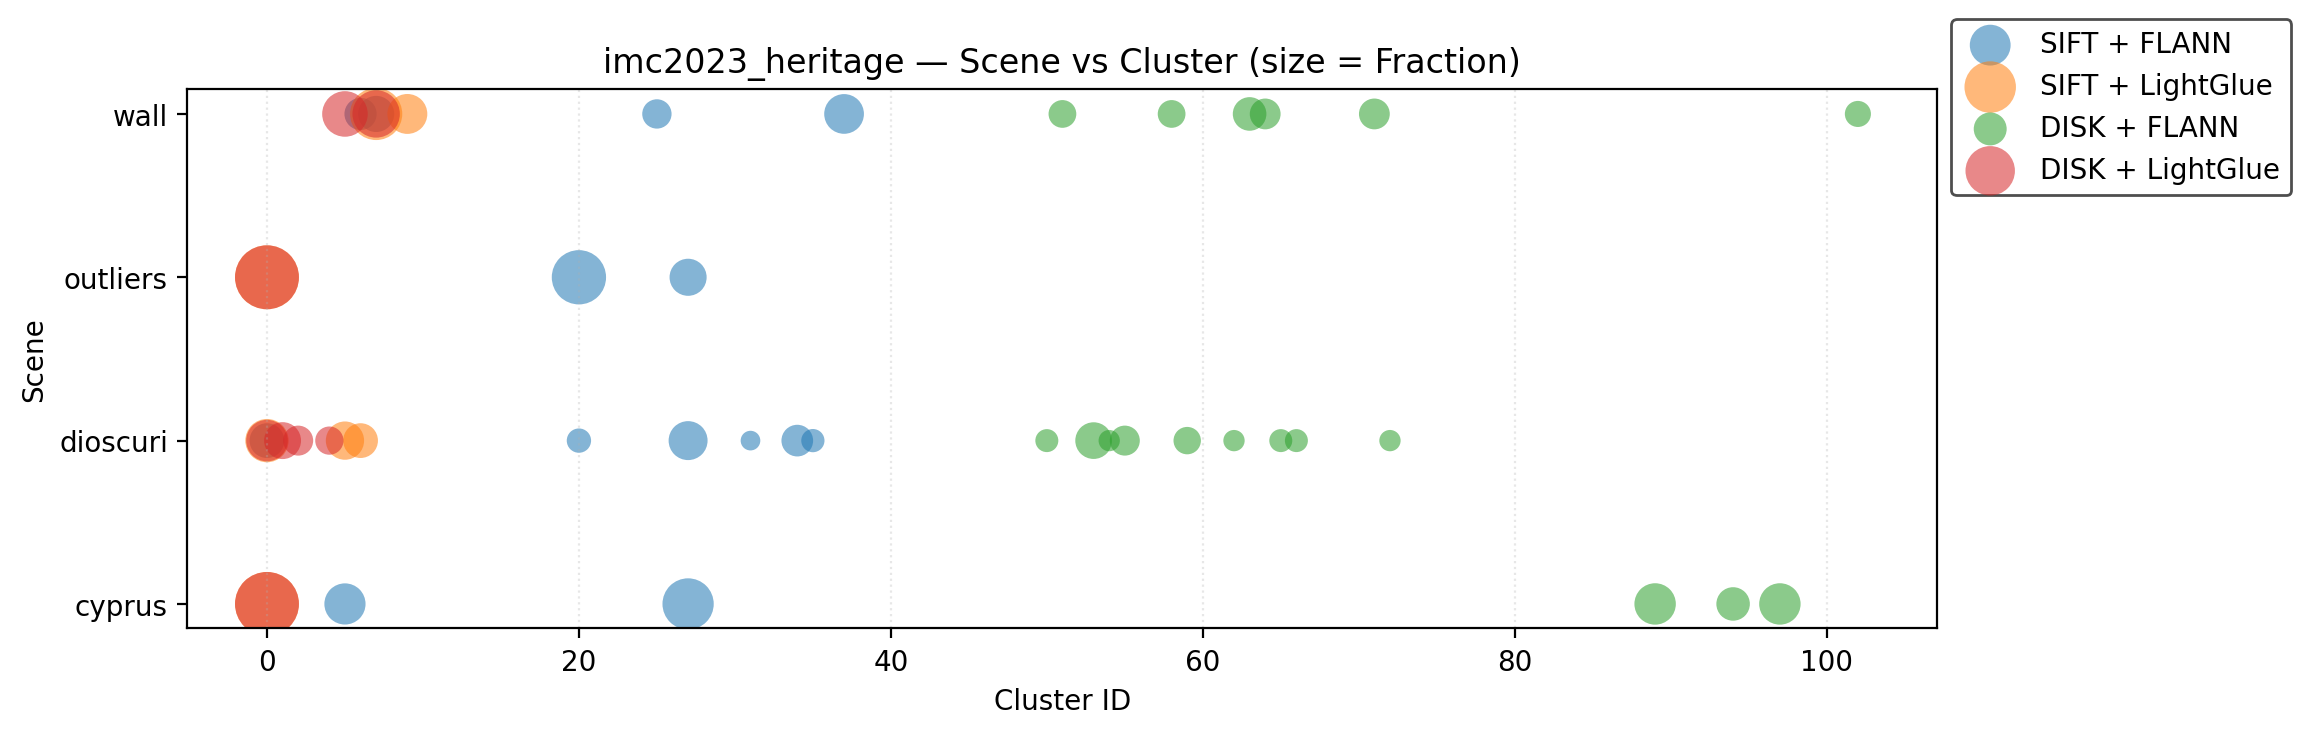
\includegraphics[width=\linewidth]{images/scene_cluster_by_dataset/imc2023_heritage.png}
% \subcaption{Dataset: imc2023\_heritage}
% \label{fig:scene-cluster-B}
% \end{minipage}

% % \vspace{0.6em}

% \begin{minipage}{\textwidth}
% \centering
% 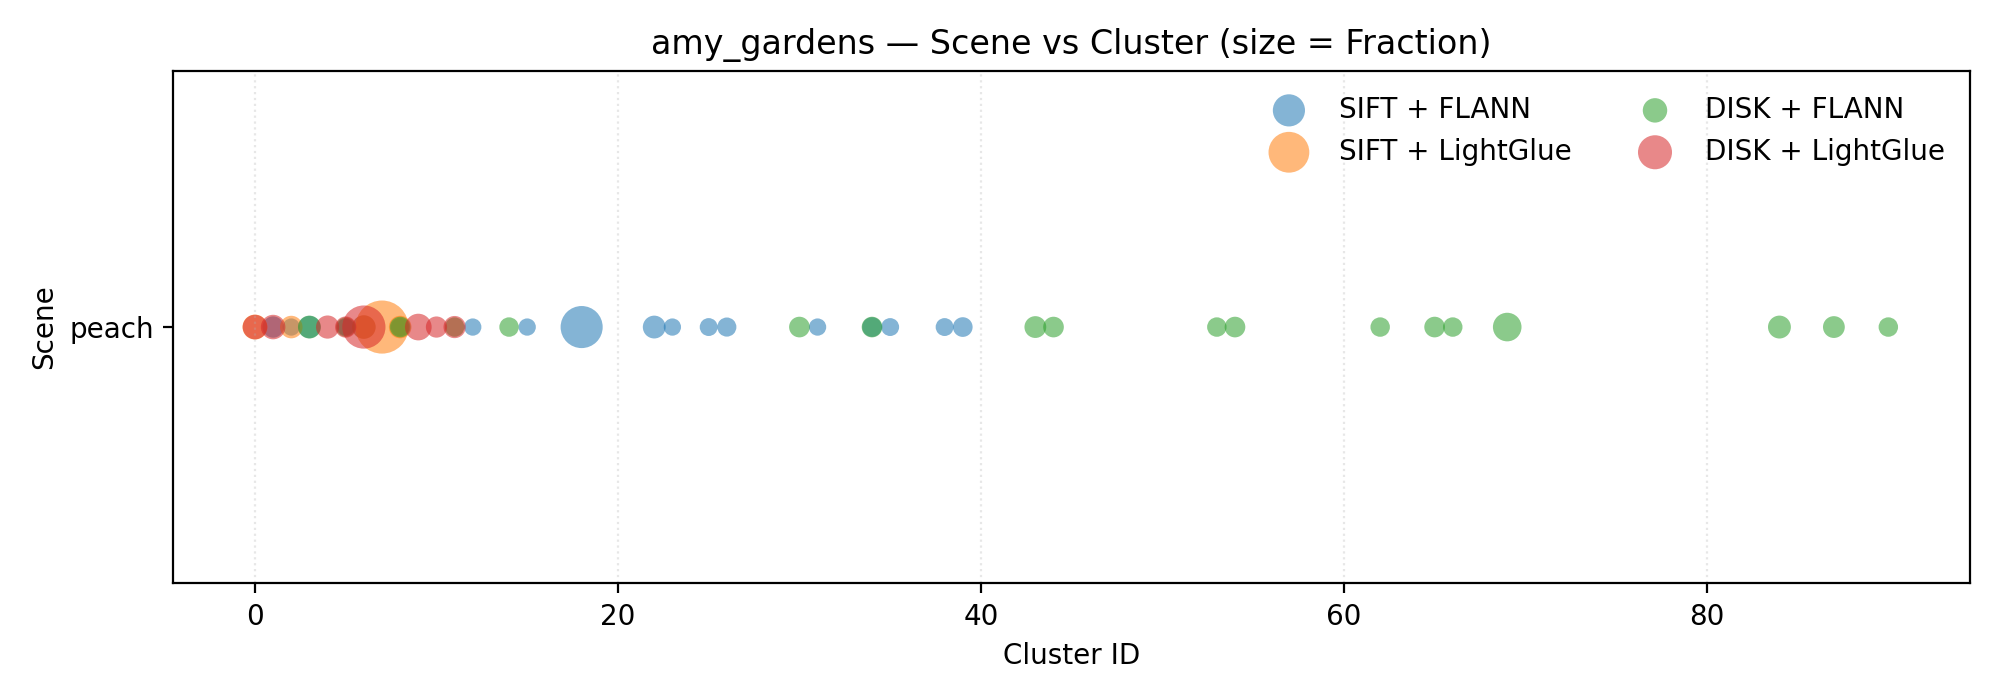
\includegraphics[width=\linewidth]{images/scene_cluster_by_dataset/amy_gardens.png}
% \subcaption{Dataset: amy\_gardens}
% \label{fig:scene-cluster-C}
% \end{minipage}
% \begin{minipage}{\textwidth}\ContinuedFloat
% \centering
% 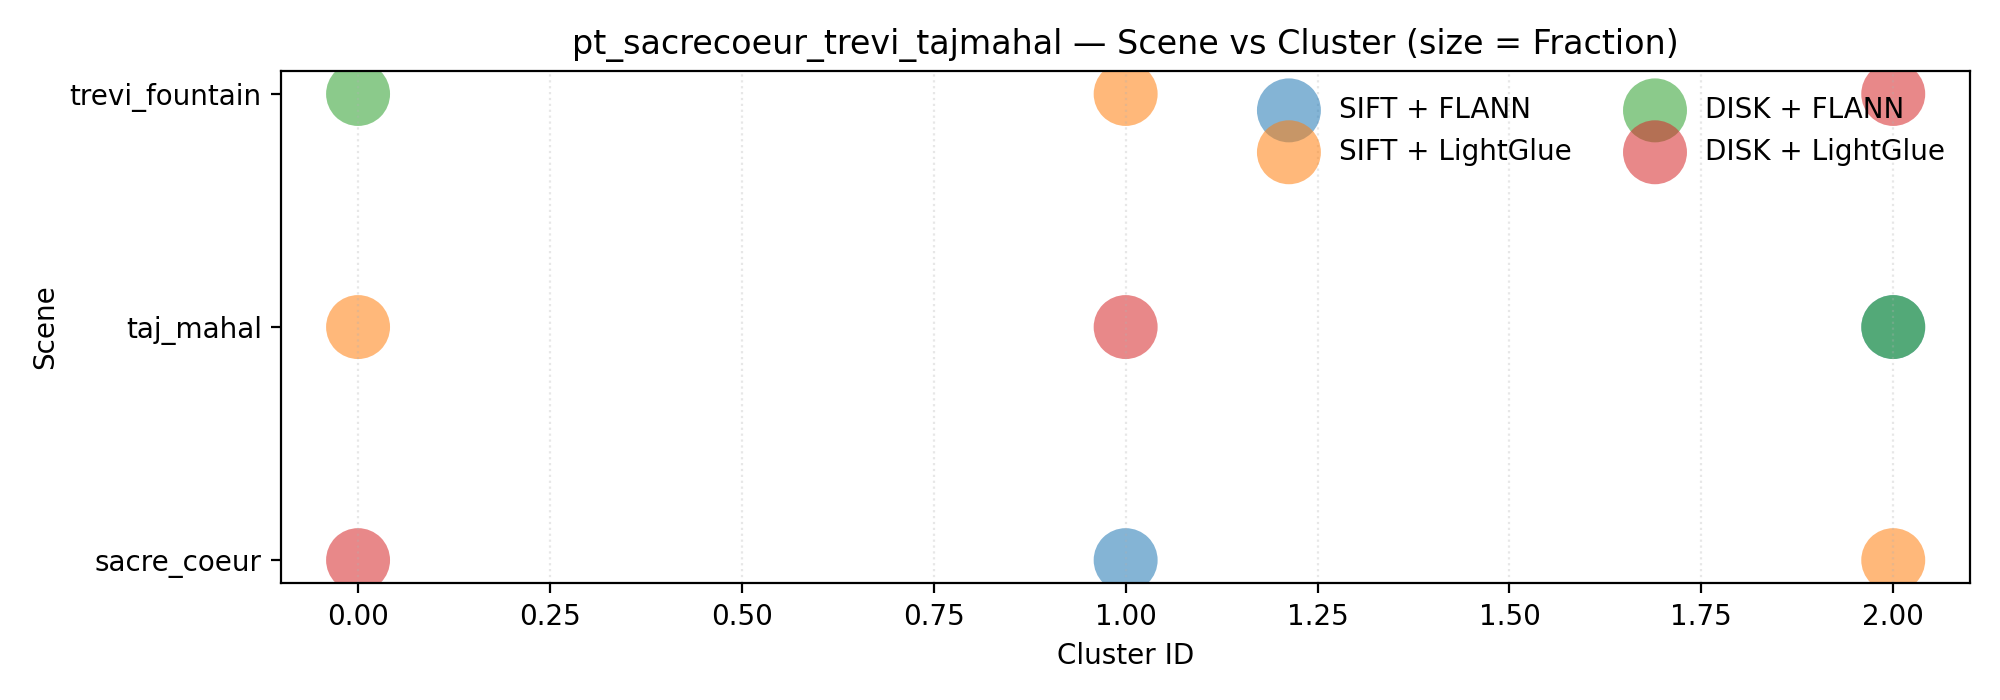
\includegraphics[width=\linewidth]{images/scene_cluster_by_dataset/pt_sacrecoeur_trevi_tajmahal.png}
% \subcaption{Dataset: pt\_sacrecoeur\_trevi\_tajmahal}
% \label{fig:scene-cluster-D}
% \end{minipage}

% \caption{Scene–cluster overlap per dataset. Each marker at (cluster, scene) encodes overlap size (fraction per scene); color denotes method. Larger, concentrated markers indicate stronger scene–cluster alignment.}
% \label{fig:scene-cluster-4up}
% \end{figure}

\begin{figure}[!htbp]
\centering
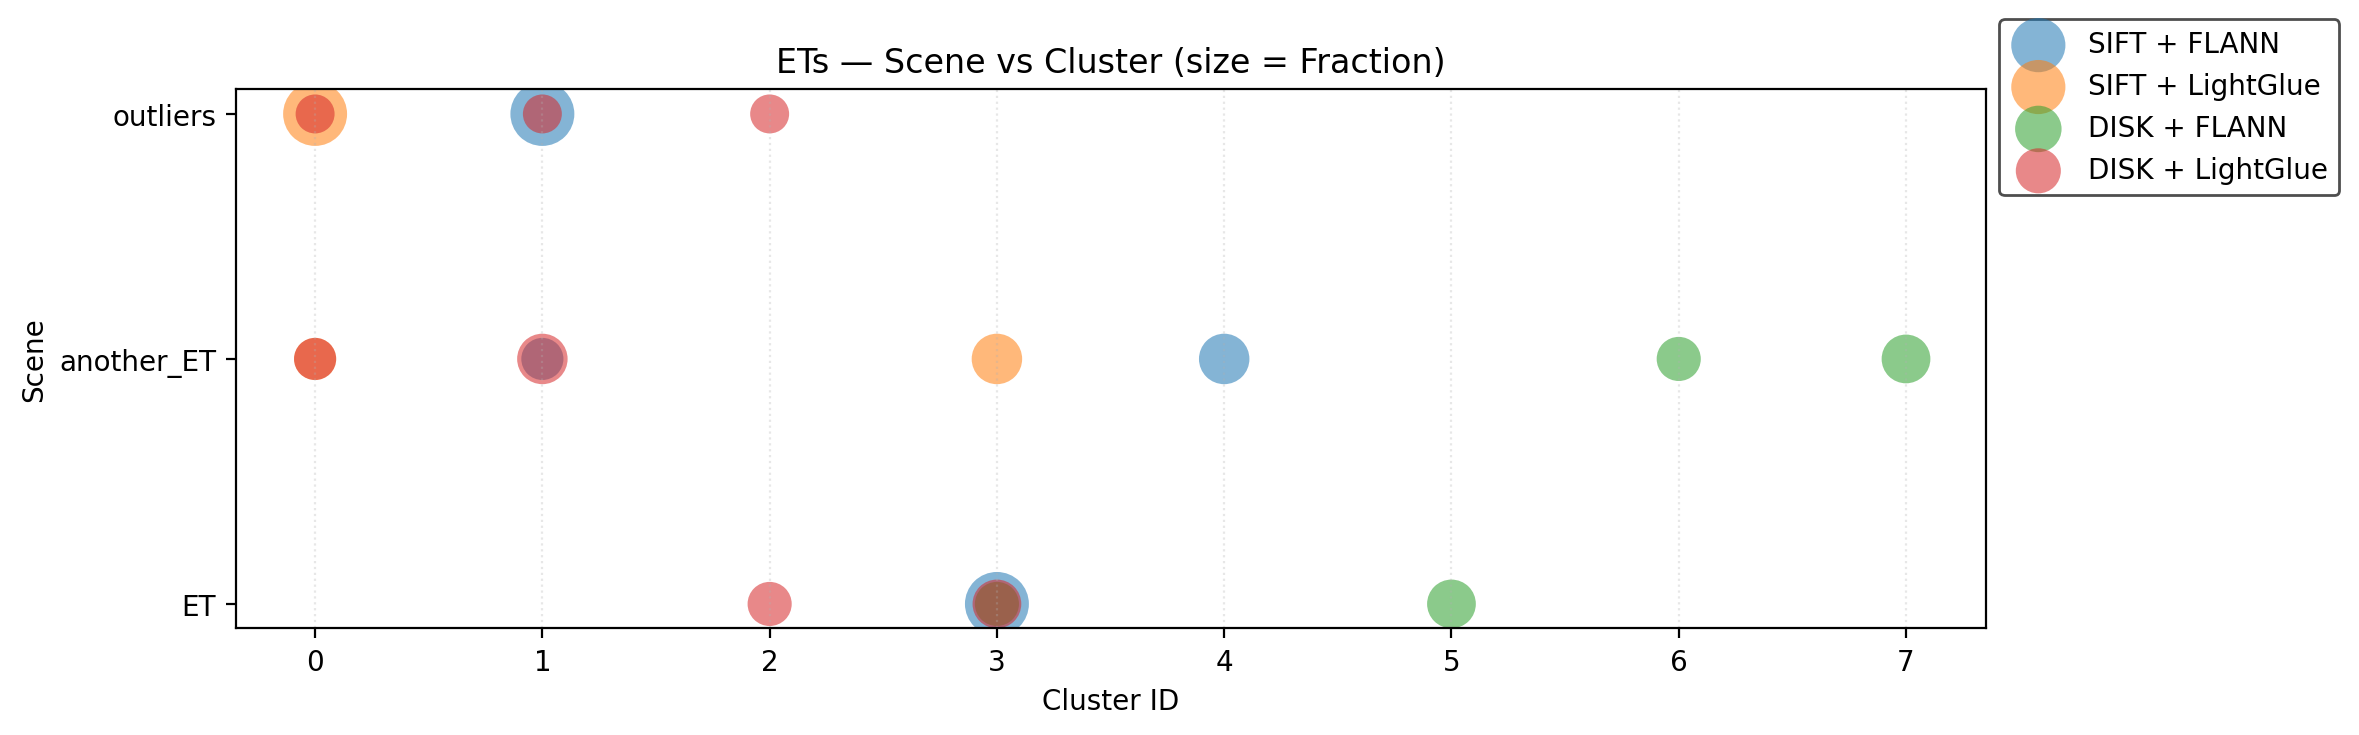
\includegraphics[width=\linewidth]{images/scene_cluster_by_dataset/ETs.png}
% \subcaption{Dataset: ETs}
% \label{fig:scene-cluster-A}

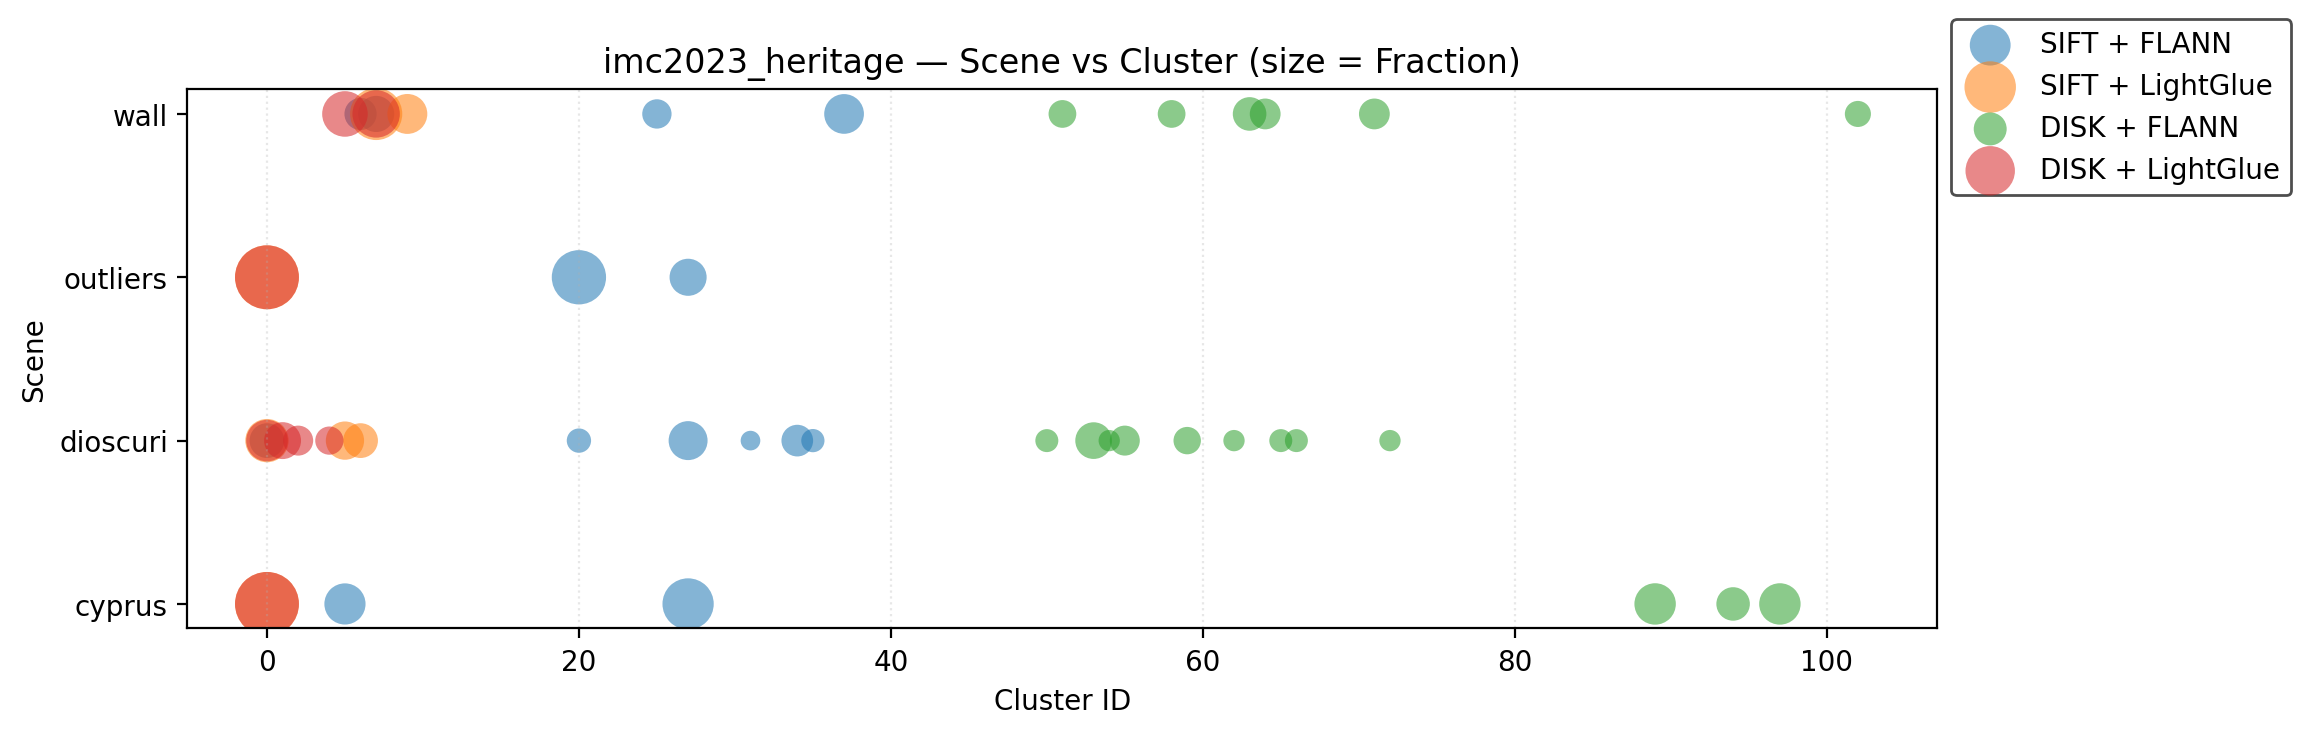
\includegraphics[width=\linewidth]{images/scene_cluster_by_dataset/imc2023_heritage.png}
% \subcaption{Dataset: imc2023\_heritage}
% \label{fig:scene-cluster-B}
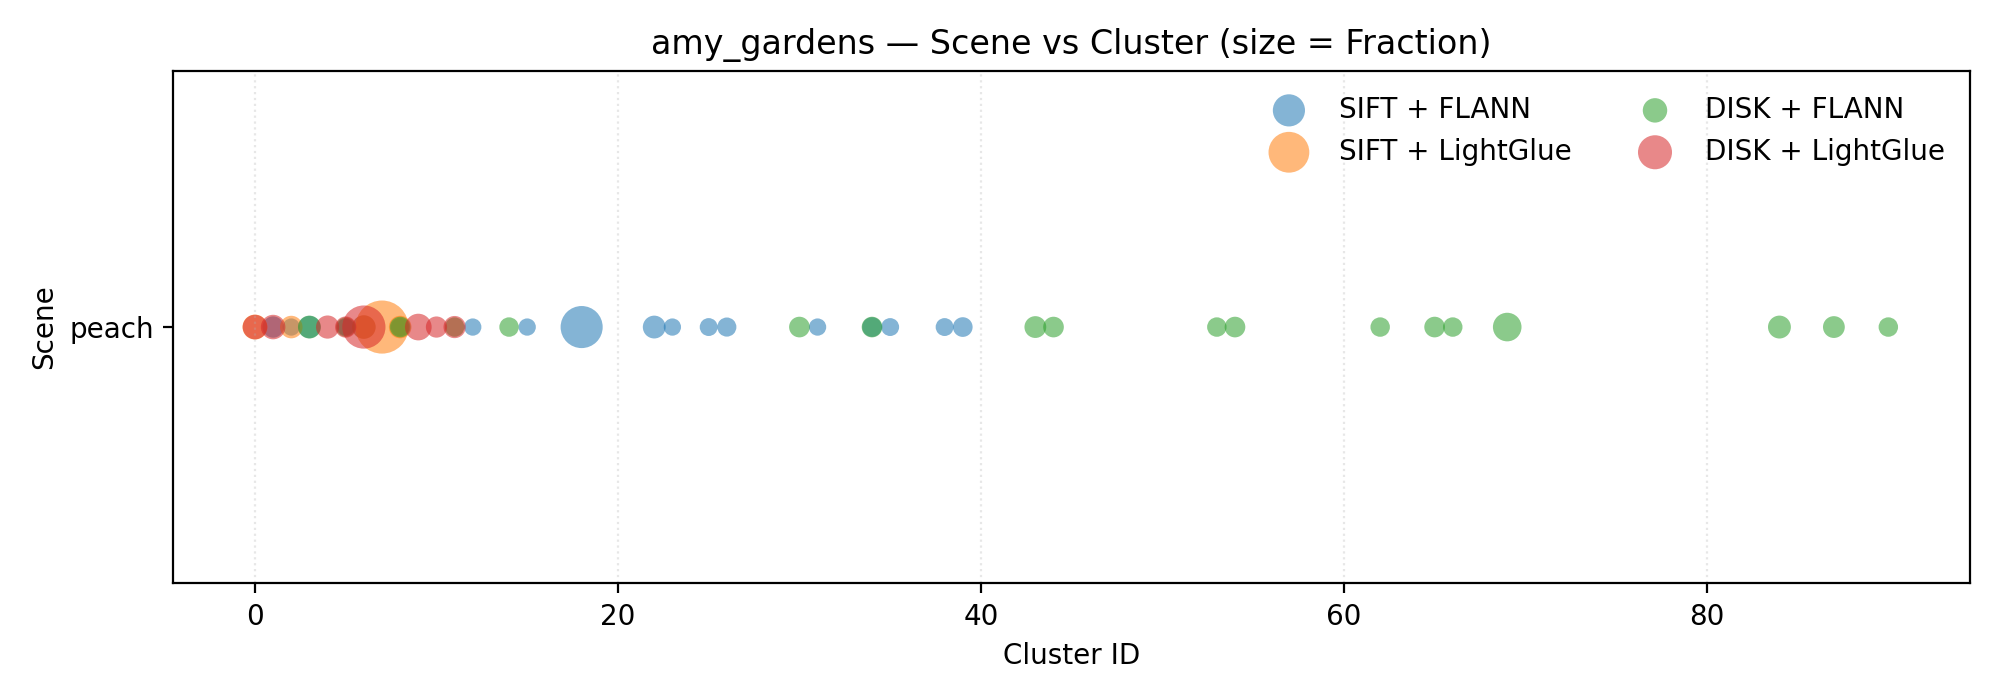
\includegraphics[width=\linewidth]{images/scene_cluster_by_dataset/amy_gardens.png}
% \subcaption{Dataset: amy\_gardens}
% \label{fig:scene-cluster-C}
\caption{Scene–cluster overlap per dataset. Each marker at (cluster, scene) encodes overlap size (fraction per scene); color denotes method. Larger, concentrated markers indicate stronger scene–cluster alignment. (Part 1)}
\end{figure}

\begin{figure}[!htbp]\ContinuedFloat
\centering
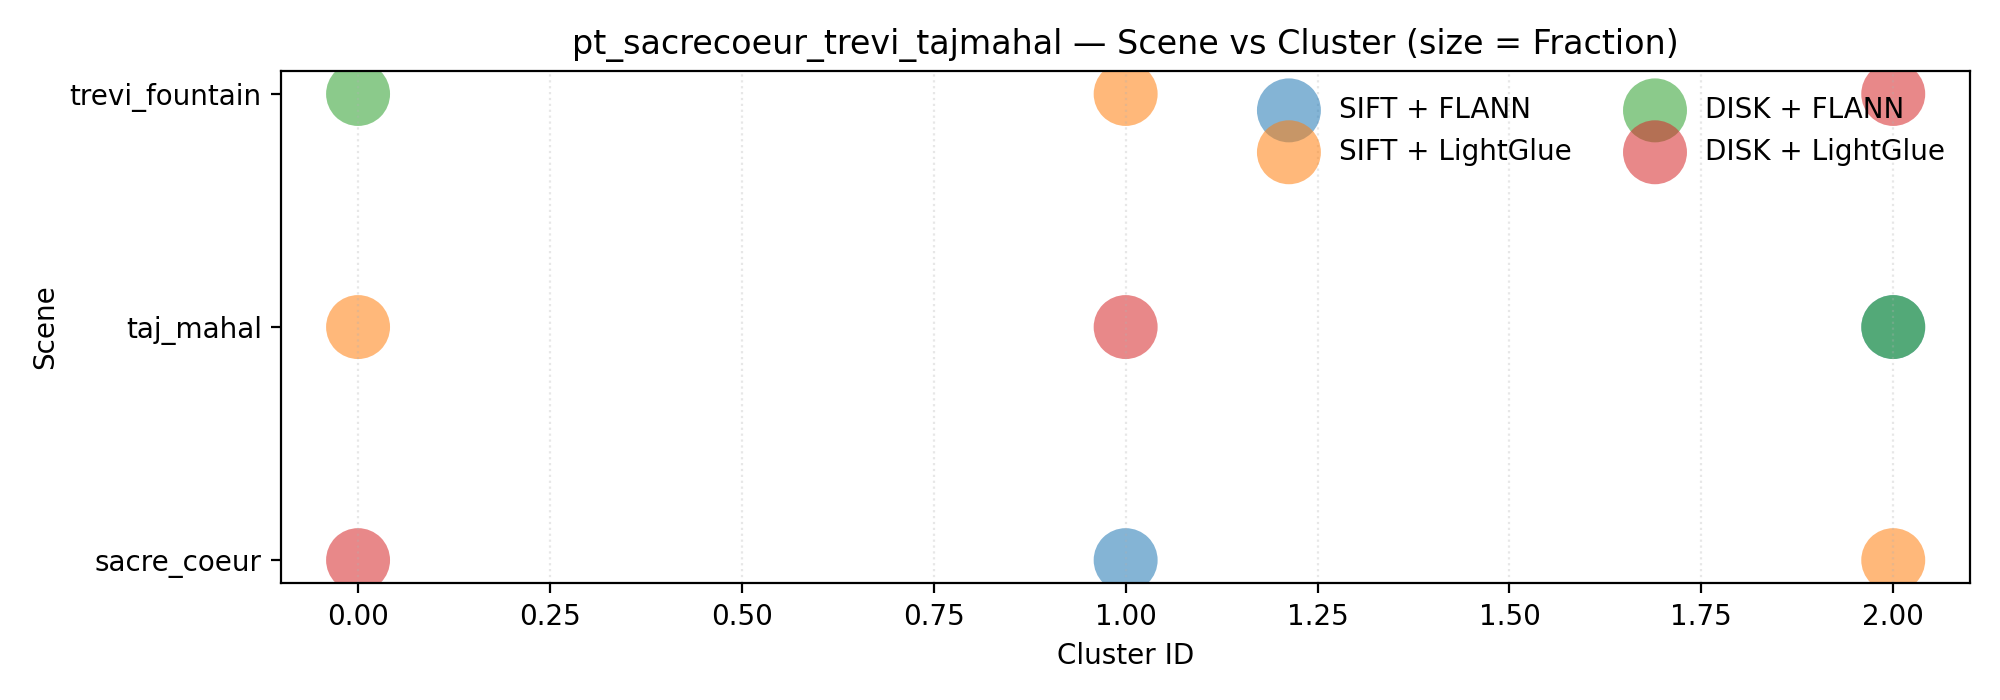
\includegraphics[width=\linewidth]{images/scene_cluster_by_dataset/pt_sacrecoeur_trevi_tajmahal.png}
% \subcaption{Dataset: pt\_sacrecoeur\_trevi\_tajmahal}

\caption{Scene–cluster overlap per dataset. Each marker at (cluster, scene) encodes overlap size (fraction per scene); color denotes method. Larger, concentrated markers indicate stronger scene–cluster alignment. (Part 2)}
\label{fig:scene-cluster-D}
\end{figure}


\subsection{Ablation: Descriptor and Matcher Choices}
Table~\ref{tab:quality-per-dataset} compares clustering quality when building clusters from different descriptor/matcher combinations. For each setting, clusters are formed from pairwise matches produced by the respective matcher and evaluated identically.
Homogeneity, Completeness, and V-Measure together characterize cluster quality with respect to ground-truth scenes. 
Homogeneity measures cluster purity (each cluster should contain only one scene); higher is better and indicates less mixing of scenes within clusters. 
Completeness measures scene fragmentation (all images from a scene should fall into the same cluster); higher is better and indicates fewer scene splits across clusters. 
V-Measure is the harmonic mean of Homogeneity and Completeness and summarizes the trade-off; it is high only when both are high.

\begin{itemize}
    \item Perfect clustering for dataset \texttt{pt\_brandenburg\_british\_buckingham}: This plot shows an ideal clustering scenario for the LightGlue methods. Each scene (e.g., buckingham\_palace) is perfectly matched to a single, pure cluster, represented by a single large marker. This indicates that these methods are highly effective for scenes with distinct, well-defined visual features and good overlap between images.
    \item Failure case for dataset \texttt{amy\_gardens}: All methods perform poorly on this dataset, forming a dense line of tiny, fragmented clusters. This suggests that the dataset contains very few valid matches between images, perhaps due to factors like significant viewpoint changes, lack of distinct visual features, or an abundance of unique, non-overlapping content. The fragmentation indicates that the clustering algorithm failed to find meaningful connections to group images. Few of the sample images from this dataset can be found in the Appendix \ref{appendix:A1}.
    % add reference for images in appendix

    \item Mixed performance for dataset \texttt{fbk\_vineyard}: This dataset highlights the different behaviors of the methods. The \texttt{vineyard\_split\_1} scene is highly fragmented by the FLANN methods, but both LightGlue methods manage to group most of its images into a single cluster. This demonstrates LightGlue's superior ability to handle more challenging, fragmented scenes.

\end{itemize}

% \begin{table} [!htbp]
% \begin{tabular}{llrrr}
\begin{longtable}{llrrr}
 &  & Homogeneity & Completeness & V-Measure \\
Dataset & Method &  &  &  \\
\midrule
\multirow[t]{4}{*}{ETs} & DISK + FLANN & 1.000 & 0.502 & 0.669 \\
 & DISK + LightGlue & 0.641 & 0.464 & 0.538 \\
 & SIFT + FLANN & 0.757 & 0.638 & 0.693 \\
 & SIFT + LightGlue & 0.319 & 0.250 & 0.280 \\
\cline{1-5}
\multirow[t]{4}{*}{amy\_gardens} & DISK + FLANN & 1.000 & 0.000 & 0.000 \\
 & DISK + LightGlue & 1.000 & 0.000 & 0.000 \\
 & SIFT + FLANN & 1.000 & 0.000 & 0.000 \\
 & SIFT + LightGlue & 1.000 & 0.000 & 0.000 \\
\cline{1-5}
\multirow[t]{4}{*}{fbk\_vineyard} & DISK + FLANN & 1.000 & 0.315 & 0.479 \\
 & DISK + LightGlue & 1.000 & 0.753 & 0.859 \\
 & SIFT + FLANN & 0.532 & 0.240 & 0.331 \\
 & SIFT + LightGlue & 1.000 & 0.767 & 0.868 \\
\cline{1-5}
\multirow[t]{4}{*}{imc2023\_haiper} & DISK + FLANN & 0.779 & 0.437 & 0.560 \\
 & DISK + LightGlue & 0.595 & 0.529 & 0.560 \\
 & SIFT + FLANN & 0.515 & 1.000 & 0.680 \\
 & SIFT + LightGlue & 0.554 & 1.000 & 0.713 \\
\cline{1-5}
\multirow[t]{4}{*}{imc2023\_heritage} & DISK + FLANN & 1.000 & 0.351 & 0.519 \\
 & DISK + LightGlue & 0.498 & 0.497 & 0.498 \\
 & SIFT + FLANN & 0.705 & 0.428 & 0.532 \\
 & SIFT + LightGlue & 0.523 & 0.551 & 0.537 \\
\cline{1-5}
\multirow[t]{4}{*}{imc2023\_theather\_imc2024\_church} & DISK + FLANN & 1.000 & 0.246 & 0.394 \\
 & DISK + LightGlue & 1.000 & 0.641 & 0.781 \\
 & SIFT + FLANN & 0.906 & 0.456 & 0.607 \\
 & SIFT + LightGlue & 0.548 & 0.381 & 0.450 \\
\cline{1-5}
\multirow[t]{4}{*}{imc2024\_dioscuri\_baalshamin} & DISK + FLANN & 1.000 & 0.401 & 0.572 \\
 & DISK + LightGlue & 0.930 & 0.491 & 0.642 \\
 & SIFT + FLANN & 0.889 & 0.475 & 0.619 \\
 & SIFT + LightGlue & 0.938 & 0.481 & 0.636 \\
\cline{1-5}
\multirow[t]{4}{*}{imc2024\_lizard\_pond} & DISK + FLANN & 1.000 & 0.394 & 0.566 \\
 & DISK + LightGlue & 0.540 & 0.351 & 0.425 \\
 & SIFT + FLANN & 0.775 & 0.303 & 0.436 \\
 & SIFT + LightGlue & 0.459 & 0.312 & 0.372 \\
\cline{1-5}
\multirow[t]{4}{*}{pt\_brandenburg\_british\_buckingham} & DISK + FLANN & 1.000 & 0.921 & 0.959 \\
 & DISK + LightGlue & 0.952 & 1.000 & 0.975 \\
 & SIFT + FLANN & 0.952 & 1.000 & 0.975 \\
 & SIFT + LightGlue & 1.000 & 1.000 & 1.000 \\
\cline{1-5}
\multirow[t]{4}{*}{pt\_piazzasanmarco\_grandplace} & DISK + FLANN & 1.000 & 0.420 & 0.591 \\
 & DISK + LightGlue & 1.000 & 1.000 & 1.000 \\
 & SIFT + FLANN & 1.000 & 1.000 & 1.000 \\
 & SIFT + LightGlue & 1.000 & 1.000 & 1.000 \\
\cline{1-5}
\multirow[t]{4}{*}{pt\_sacrecoeur\_trevi\_tajmahal} & DISK + FLANN & 1.000 & 1.000 & 1.000 \\
 & DISK + LightGlue & 1.000 & 1.000 & 1.000 \\
 & SIFT + FLANN & 1.000 & 1.000 & 1.000 \\
 & SIFT + LightGlue & 1.000 & 1.000 & 1.000 \\
\cline{1-5}
\multirow[t]{4}{*}{pt\_stpeters\_stpauls} & DISK + FLANN & 1.000 & 0.611 & 0.758 \\
 & DISK + LightGlue & 1.000 & 1.000 & 1.000 \\
 & SIFT + FLANN & 1.000 & 1.000 & 1.000 \\
 & SIFT + LightGlue & 0.000 & 1.000 & 0.000 \\
% \end{tabular}
\caption{Cluster quality per dataset and method}
\label{tab:quality-per-dataset}
% \end{table}
\end{longtable}

% \subsection{Visualization of the clusters}
% We try to visualy 

\end{document}
